
\subsection{Results I:  The Experiment}

\label{sec:results}

This section reports results of analyzing 945 Jar libraries extracted
from Debian 6.0 Squeeze to answer the research questions formulated in
Section~\ref{sec:method}.  By treating version and name information
encoded in the 945 Jar files as a good approximation of ground truth,
we can compare our signature-based Bertillonage technique against a
baseline technique.

All our techniques consider only the top match according to similarity,
as described in Section~\ref{sec:sim}.  Often the top similarity score
is shared by several artifacts in our corpus.  As the results show, 2-way,
3-way, and 4-way ties for best similarity are the norm, rather than the
exception, and we even observed an 86-way tie.  However, to understand
what we mean by a `tie,' we must mention briefly what we consider `a single
artifact.'  Our earlier exploration of the Maven 2 corpus (see
Section~\ref{sec:mavenExplore}) shows incredible redundancy and duplication
of archives.  Users are likely not interested in knowing all two hundred
path locations of an identical artifact.  We filter out these duplications
and instead only report ties that either have a different SHA1 binary
fingerprint than other matches in the tie, or a different name.  

In some cases choosing a top match based on the inclusion metric rather
than similarity performs better.  To keep our experiment simple, we
consider these to be wrong matches.  We anticipate future researchers
will improve on our results by tuning the match criteria to factor in
both similarity and inclusion scores when selecting the `top' match,
perhaps at a cost of larger `ties.'


\subsubsection{The Baseline:  Binary Fingerprint Matches}

\begin{table}[h]
  \centering
\begin{tabular}[htbp]{l|r|lll|rrr}
  sha1-of-class/Debian-945   &              & \multicolumn{3}{c|}{\textbf{Similarity}}  & \multicolumn{3}{c}{\textbf{\# of Ties}} \\
  \textbf{Type of Match}     & Count        & Min   & Mdn    & Max   & Min  & Mdn  & Max  \\
\hline
  \emph{HQ1.} Identical archive          &   2          & 1.0   & 1.0    & 1.0   & 1    & 1    &  1   \\
  \emph{HQ2.} Identical contents         & 201          & 1.0   & 1.0    & 1.0   & 1    & 1    & 35   \\
  \emph{HQ3.} Expected match             & 131          & 0.014 & 0.680  & 0.997 & 1    & 1    & 13   \\
  \emph{HQ4.} Version off by final digit &  49          & 0.033 & 0.500  & 0.977 & 1    & 1    &  4   \\
  & & & & & & & \\
  \emph{LQ1.} Version off by many digits &  85          & 0.001 & 0.116  & 0.964 & 1    & 1    & 25   \\
  \emph{LQ2.} Not useful                 &  22          & 0.003 & 0.025  & 0.206 & 1    & 1    & 18   \\
\hline
  \textbf{Total:} \hspace{8em} (52\%) & 490   & \multicolumn{3}{c|}{Average: 0.685}  & \multicolumn{3}{c}{Average: 2.4} \\
\end{tabular}
  \caption{sha1 of *.class - the technique we need to beat, otherwise what's the point! (945 debian jars)}
  \label{tab:debianSha1OfClass}
\end{table}


Table \ref{tab:debianSha1OfClass} shows the results of our baseline technique, a straightforward SHA1 index of
Jar files and class files.
Slighly over half the Debian sample, 490 jars out of 945 (52\%), contained one or more class files that were
identical to a class file in the Maven corpus.

Only 2 out of the 945 jar files proved to be identical complete archive copies from the Maven corpus
(row \emph{HQ1}).
We suspect the main reason for such a low match percentage (less than 0.5\%) in this category
may be Debian's policy of recompiling all jar files from original sources.
Jar files record timestamps of contained files, and Java class files tend to have timestamps
set to the moment they were compiled.  This alone will cause Debian jar files
to differ, at least in a few bytes, from their Maven counterparts.matches
A further 201 out of the 945 jar files matched with identical contents (row \emph{HQ2}).
These 201 matches, while externally different, were internally identical with respect to contained class files.
Of course the 2 identical Jar files also matched according to contents.

A remaining 287 Jar files had partial matches, with similarity scores less than 1.0.
Of these, 180 matches, when evaluated against our ground truth, scored as high quality matches (rows \emph{HQ3} and \emph{HQ4}),
and 107 matches scored as low quality matches (rows \emph{LQ1} and \emph{LQ2}).
In most cases the matches provided good leads with respect to provenance.

[Talk about medians.  Talk about match frequencies.]

Finally, for 455 jars, there were no matches at all using the binary fingerprint technique.



\begin{table}[h]
  \centering
\begin{tabular}[htbp]{l|r|lll|rrr}
  bin2bin/Debian             &                & \multicolumn{3}{c|}{\textbf{Best Match Score}}  & \multicolumn{3}{c}{\textbf{\# of Matches}} \\
  \textbf{Type of Match}     & Count        & Min   & Mdn    & Max   & Min  & Mdn  & Max  \\
  \hline
  \emph{HQ1.} Exact (sha1 of jar)        &   2          & 1.0   & 1.0    & 1.0   & 1    & 1.5  &  2   \\
  \emph{HQ2.} Exact (sha1 of *.class)    & 201          & 1.0   & 1.0    & 1.0   & 1    & 3    & 86   \\
  \emph{HQ3.} Expected match             & 443          & 0.014 & 1.0    & 1.0   & 1    & 2    & 30   \\
  \emph{HQ4.} Version off by final digit &  65          & 0.038 & 0.889  & 1.0   & 1    & 1    & 23   \\
  & & & & & & & \\
  \emph{LQ1.} Version off by many digits &  66          & 0.015 & 0.414  & 1.0   & 1    & 1    & 14   \\
  \emph{LQ2.} Not useful                 &  16          & 0.002 & 0.027  & 0.807 & 1    & 1    &  4   \\
  \hline
  \textbf{Total:} \hspace{8em}    (84\%) &  793   & \multicolumn{3}{c|}{Average: 0.890}  & \multicolumn{3}{c}{Average: 3.5} \\
\end{tabular}
  \caption{bin2bin bertillionage - our signature based approach applied to 945 debian jars}
  \label{tab:debianBin2Bin}
\end{table}


\subsubsection{Bertillonage, Binary-to-Binary Anchored Signature}


\textbf{Class Signature Index, Binary-To-Binary Match} (bin2bin)

Table~\ref{tab:debianBin2Bin} shows the detailed results of our binary-to-binary
bertillonage-based technique.

Anchored class signatures never disagreed with the byte-oriented techniques:
whenever byte-oriented techniques found perfect 1.0 similarity matches,
the bin2bin index did as well.



\subsubsection{Bertillonage, Binary-to-Source Anchored Signature}


\begin{table}[h]
  \centering
\begin{tabular}[htbp]{l|r|lll|rrr}
  bin2src/Debian                         &       & \multicolumn{3}{c|}{\textbf{Best Match Score}}  & \multicolumn{3}{c}{\textbf{\# of Matches}} \\
  \textbf{Type of Match}                 & Count & Min   & Mdn   & Max   & Min & Mdn  & Max  \\
  \hline
  \emph{HQ1.} Exact (sha1 of jar)        & \multicolumn{1}{c|}{\emph{n/a}} & & \emph{n/a} & & & \emph{n/a} &  \\
  \emph{HQ2.} Exact (sha1 of *.class)    & & & & & & & \\
  \emph{HQ3.} Expected match             & 443   & 0.001 & 1.0   & 1.0   & 1   & 2    & 77   \\
  \emph{HQ4.} Version off by final digit &  84   & 0.018 & 0.750 & 1.0   & 1   & 1    &  2   \\
  & & & & & & & \\
  \emph{LQ1.} Version off by many digits & 109   & 0.001 & 0.326 & 1.0   & 1   & 1    & 20   \\
  \emph{LQ2.} Not useful                 &  24   & 0.002 & 0.136 & 0.886 & 1   & 1.5  & 20   \\
  \hline
  \textbf{Total:} \hspace{8em}    (70\%) &  660  & \multicolumn{3}{c|}{Average: 0.773}  & \multicolumn{3}{c}{Average: 2.9} \\
\end{tabular}
  \caption{bin2src bertillionage - our signature based approach applied to 945 debian jars}
  \label{tab:debianBin2Src}
\end{table}


\textbf{Class Signature Index, Binary-To-Source Match} (bin2src)

Table~\ref{tab:debianBin2Src} shows the detailed results of our binary-to-source
bertillonage-based technique.




\subsection{Results II:  The Case Study}


\begin{table}[h]
  \centering
\begin{tabular}[htbp]{l|r|lll|rrr}
  sha1-of-class/Industry     &              & \multicolumn{3}{c|}{\textbf{Best Match Score}}  & \multicolumn{3}{c}{\textbf{\# of Matches}} \\
  \textbf{Type of Match}     & Count        & Min   & Mdn    & Max   & Min  & Mdn  & Max  \\
  \hline
  \emph{HQ1.} Exact (sha1 of jar)        & 54           & 1.0   & 1.0    & 1.0   & 1    & 2    & 14   \\
  \emph{HQ2.} Exact (sha1 of *.class)    &  9           & 1.0   & 1.0    & 1.0   & 1    & 1    &  5   \\
  \emph{HQ3.} Expected match             &  4           & 0.006 & 0.758  & 0.965 & 1    & 1.5  &  4   \\
  \emph{HQ4.} Version off by final digit &  7           & 0.016 & 0.500  & 0.962 & 1    & 1    & 12   \\
  & & & & & & & \\
  \emph{LQ1.} Version off by many digits &  1           & 0.038 & 0.038  & 0.038 & 1    & 1    &  1   \\
  \emph{LQ2.} Not useful                 &  2           & 0.002 & 0.031  & 0.059 & 1    & 1    &  1   \\
  \hline
  \textbf{Total:} \hspace{8em}    (95\%) &  77   & \multicolumn{3}{c|}{Average: 0.903}  & \multicolumn{3}{c}{Average: 2.8} \\
  & & & & & & & \\
  & & & & & & & \\

\end{tabular}
  \caption{sha1 of *.class - the technique we need to beat, otherwise what's the point!}
  \label{tab:bankSha1OfClass}
\end{table}


\begin{table}[h]
  \centering
\begin{tabular}[htbp]{l|r|lll|rrr}
  bin2bin/Industry           &              & \multicolumn{3}{c|}{\textbf{Best Match Score}}  & \multicolumn{3}{c}{\textbf{\# of Matches}} \\
  \textbf{Type of Match}     & Count        & Min   & Mdn    & Max   & Min  & Mdn  & Max  \\
  \hline
  \emph{HQ1.} Exact (sha1 of jar)        & 54           & 1.0   & 1.0    & 1.0   & 1    & 3    & 16   \\
  \emph{HQ2.} Exact (sha1 of *.class)    &  9           & 1.0   & 1.0    & 1.0   & 1    & 1    &  9   \\
  \emph{HQ3.} Expected match             &  6           & 0.933 & 0.994  & 1.0   & 1    & 1    &  2   \\
  \emph{HQ4.} Version off by final digit &  8           & 0.133 & 0.915  & 1.0   & 1    & 1    & 12   \\
  & & & & & & & \\
  \emph{LQ1.} Version off by many digits &  1           & 0.132 & 0.132  & 0.132 & 1    & 1    &  1   \\
  \emph{LQ2.} Not useful                 &  3           & 0.002 & 0.023  & 0.068 & 1    & 1    &  1   \\
  \hline
  \textbf{Total:} \hspace{7.5em} (100\%) &  81   & \multicolumn{3}{c|}{Average: 0.926}  & \multicolumn{3}{c}{Average: 3.6} \\
\end{tabular}
  \caption{bin2bin bertillionage - our signature based approach}
  \label{tab:bankBin2Bin}
\end{table}


\begin{table}[h]
  \centering
\begin{tabular}[htbp]{l|r|lll|rrr}
  bin2src/Industry                       &              & \multicolumn{3}{c|}{\textbf{Best Match Score}}  & \multicolumn{3}{c}{\textbf{\# of Matches}} \\
  \textbf{Type of Match}                 & Count        & Min   & Mdn    & Max   & Min  & Mdn  & Max  \\
  \hline
  \emph{HQ1.} Exact (sha1 of jar)        & \multicolumn{1}{c|}{\emph{n/a}} & & \emph{n/a} & & & \emph{n/a} &  \\
  \emph{HQ2.} Exact (sha1 of *.class)    & & & & & & & \\
  \emph{HQ3.} Expected match             &  41          & 0.168 & 1.0    & 1.0   & 1    & 1    &  2   \\
  \emph{HQ4.} Version off by final digit &  14          & 0.054 & 0.865  & 1.0   & 1    & 1    & 12   \\
  & & & & & & & \\
  \emph{LQ1.} Version off by many digits &  12          & 0.061 & 0.491  & 1.0   & 1    & 1    &  1   \\
  \emph{LQ2.} Not useful                 &   1          & 0.068 & 0.068  & 0.068 & 1    & 1    &  1   \\
  \hline
  \textbf{Total:} \hspace{8em}    (84\%) &  68   & \multicolumn{3}{c|}{Average: 0.812}  & \multicolumn{3}{c}{Average: 1.5} \\
\end{tabular}
  \caption{bin2src bertillionage - our signature based approach}
  \label{tab:bankBin2Src}
\end{table}



\subsection{How Fast is it?}

All analysis was performed on 
a dual-core Intel Core i3 2.26ghz laptop with 8GB or RAM running Debian 6.0 and PostgreSQL 8.4.

creating source signatures on this laptop:  330/second.

creating binary signatures:  3,450/second.


sha1-of-jar: the index entries behind these two matches used the least space, and the queries required the least time to execute.

sha1-of-classes:  These require the same amount of space as our bertillonage approaches (the size
of a SHA1 signature, 20 bytes per file).  Index creation is fast:  for each
file we run a byte scan through a fingerprinting algorithm.
Index queries should perform similar to the bertillonage techniques, since
the query structure is identical, but in practice they run faster, due in part
to the lower frequency of matches (e.g. 2.4 top matches per query compared to
3.5 for bin2bin).  This makes sense, since any change to a source file,
even a new comment (and in some cases, a different compiler),
and certainly any code change, will perturb its
compiled binary representation, in turn altering its fingerprint, and precluding
the match.
This stands in sharp contrast to the bertillonage class signatures, which are only perturbed by functional
changes ``outside the curly braces,'' and thus are subject to change by a much smaller set of 
developer activities.

bin2bin: Like sha1-of-classes, these required 20 bytes
of space per file, since we ran the class signature through SHA1 before storing
it in our index.
Using the asm.jar byte-code analysis library, we were able to create our index at a
rate of 300-classes-per-second, slower than a simple SHA1 of each file, but fast enough.
For processing provenance queries, this approach was 20\% to 30\% slower for each query than
sha1-of-classes, but answers were both more likely, and more likely to be exact matches.
This increased match quality came at a cost though:  with the byte-oriented approaches,
a 1.0 match was always authoritative, whereas with this approach a small number of 1.0 matches, when
compared to our ground truth, proved to be false.



\begin{table}[h]
  \centering
\begin{tabular}[htbp]{l|rrr|rrr}
                                    & \multicolumn{3}{c|}{\textbf{Signatures + Rows}}  & \multicolumn{3}{c}{\textbf{Seconds}} \\
  \textbf{Provenance Technique}     & Mdn   & Avg    & SD    & Mdn  & Avg  & SD  \\
  \hline
  sha1 of jar                       &  3.0  &   2.9  &   1.1 & 0.1  & 0.1  & 0.0   \\
  fingerprint                       & 57.0  & 151.8  & 259.7 & 0.2  & 0.5  & 1.0  \\
  signatures bin2bin                & 77.5  & 187.8  & 290.7 & 0.3  & 0.7  & 1.3   \\
  signatures bin2src                & 53.0  & 132.3  & 237.3 & 0.3  & 0.5  & 0.6   \\
  \hline
\end{tabular}
  \caption{Performance comparison of the 4 techniques processing all Jars (945 Debian + 81 Industry).  Direct sha1 of the jar is the fastest, since
the query is very small (a single sha1) and the results are also very small (at most 6 rows).   Bin2bin is the slowest,
with potentially large queries containing many signatures, and large sets of rows in the results.}
  \label{tab:perfSummary}
\end{table}



Even though bin2bin is the slowest, 75\% of the queries
respond within 1.2 seconds.


\begin{figure}[h]
  \centering
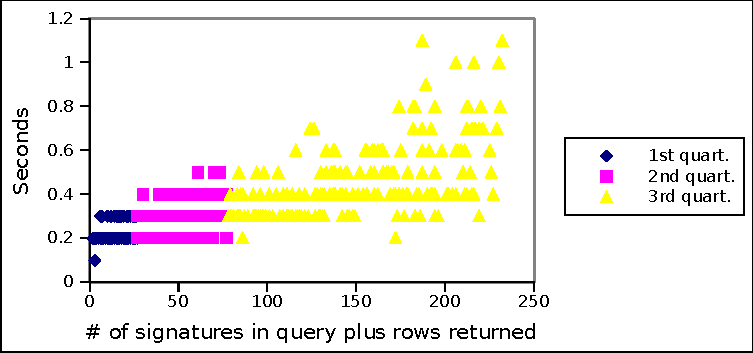
\includegraphics[width=\columnwidth]{plots/performance-bin2bin-1st-3-quartiles.pdf}
  \label{fig:perfBin2Bin3quartiles}
\end{figure}


\begin{figure}[h]
  \centering
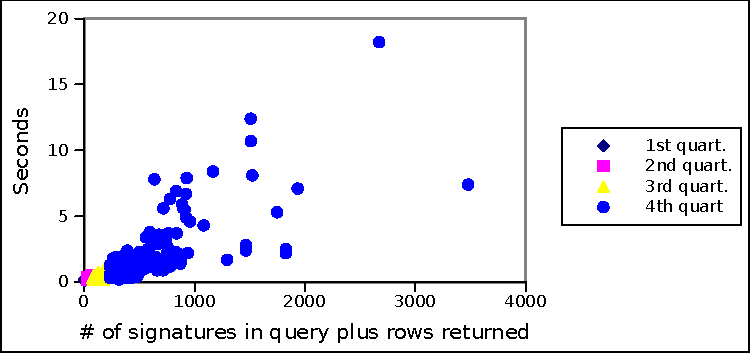
\includegraphics[width=\columnwidth]{plots/performance-bin2bin-all-4-quartiles.pdf}
  \label{fig:perfBin2Bin}
\end{figure}



\subsection{Summary and Answers}

\begin{figure}[ht]
\begin{minipage}[b]{0.5\linewidth}
\centering
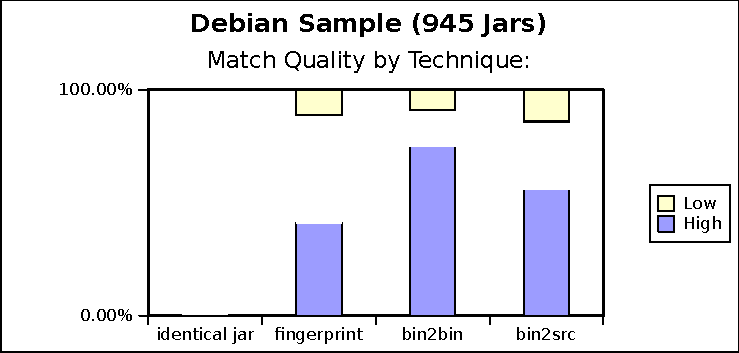
\includegraphics[width=\columnwidth]{plots/debianMatchQuality.pdf}
\label{fig:debianMatchQual}
\end{minipage}
\hspace{0.5cm}
\begin{minipage}[b]{0.5\linewidth}
\centering
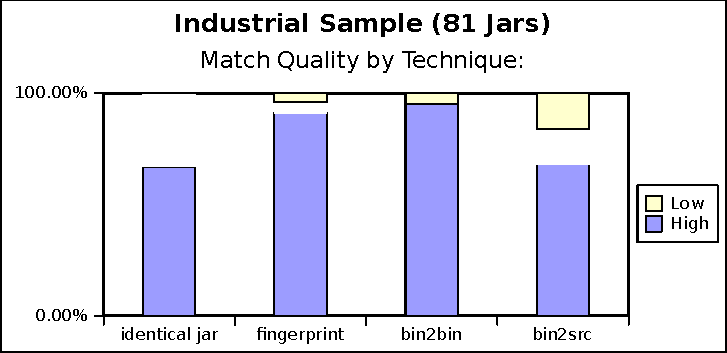
\includegraphics[width=\columnwidth]{plots/industryMatchQuality.pdf}
\label{fig:industryMatchQual}
\end{minipage}
\end{figure}



\subsubsection{RQ1, \rqOne}

\begin{hassanbox}
\textbf{RQ1:} In our study we considered two index approaches:  byte-oriented, and bertillonage-oriented.
The answer, perhaps unsurprisingly, is that both approaches have important benefits.
With the byte-oriented approaches, a 1.0 match is always authoritative, whereas with
our signature techniques (and presumably any bertillonage approach), even a 1.0 match could be false.
Since performance and storage costs imposed by each index are relatively small
(both in index creation, and query execution), a hybrid approach, combining both strategies,
offers the best solution, in so far as the experiments conducted in this study show.
By adopting a hybrid approach, implementors can benefit from the perfect certainty
offered by the byte oriented approaches, while also enjoying the improved match quality
we observed in our bertillonage approaches.
\end{hassanbox}



\subsubsection{RQ2, \rqTwo}

\begin{hassanbox}
\textbf{RQ2:} \jad{rough notes for now...} 

\begin{itemize}


\item Debian sample shows that an imperfect corpus can still provide many useful provenance ansers.
      The fact this Debian sample is arguably more challenging from a provenance perspective
      than what we might expect to observe in nature further strengthens this claim.
      (e.g, Debian patches sources, uses less common compilers, and has a policy of recompiling).

\item The industry case study shows how the corpus's own context is important to consider,
      independent of the corpus's completeness.
      In this particular example, since the Maven2 repository serves as the main dependency
      resolver for this particular company, by using the same pool from which the company is obtaining
      its libraries, we significantly boost the power of the byte-oriented techniques.
      We also wonder if the company is less likely to consider libraries not already present in Maven2,
      since such are probably inconvenient for developers to integrate into their existing environments.
                                                                   
\item Our bin2src experiment sheds some light on how an even further degraded corpus might
      impact a provenance method.  Source signatures in Maven are 2 times less common, and
      yet the results in our bin2src experiments were suprisingly decent.

\end{itemize}

\end{hassanbox}



\subsubsection{RQ3, \rqThree}

\begin{itemize}
\item Sha1 is not useful. All matches in Maven are binaries.
\end{itemize}

Results:

\begin{itemize}
\item 1 same name but .zip instead of .jar (Jaccard 1)
\item 32 Same name, including -source (max 1.0, min 0.85, median 1.0)
\item 7 variations of name. Max 1.0, min 0.609, median 0.952. For
  example: sun-jaxws-2.1.4-20080502-rt and jaxws-rt-2.1.4;19;
\item 23, variations of version.. We also checked the Inclusion in
  this one: max 1.0, min 0.113, median 0.929). We checked every one
  of them and they really looked like different variations in version
  even those with the lowest Jaccard jdom-1.0.jar and
  jgom-1.1-sources, with In. 113, and Jaccard .061, the lowest)
\item 5 False positive (not matched): Min;0.068, Max;0.225,
  Median;0.200, but even their inclusion is very  low: (Min;0.068,
  Max;0.225, Median;0.186).
\item 13 not found. 
\item For 60, there was only 1 match, for the remainder 21, the min was 2, max, 11, with median of 3. Really narrowing the searching space.
\item Results changed: now only 20 \emph{1.00} match is a single match, but median for single match is 2
\end{itemize}


We suspect two factors are contributing to the inferior performance.
First, our corpus contains only $4$ million Java source files compared
to almost $27$ million compiled class files.  This results in many fewer
source archives available for matching.  For example, batik-util-1.6.jar
matched no source archives, and yet for RQ1 the same jar file matched
$15$ distinct binary archives, ranging from similarity $1.0$ down to
$0.006$.


\begin{hassanbox}
\textbf{RQ3:} \jad{rough notes for now...} 

\begin{itemize}

\item Our bin2src experiment showed we can find sources.

\item But fundamental problems about source archives pose difficult obstacles in this area
      (e.g., unit tests, code generation, bytecode manipulation such as aspect-oriented-programming, etc.)

\item In RQ1 we propose a hybrid approach, perhaps we can offer the same suggestion here:
      binary provenance bridging.  The binary-to-binary techniques often perform very well,
      and once binary provenance information is obtained, locating a project's website, and downloading
      the corresponding source code may very well be a simple, straighforward, and ultimately
      much more robust technique compared
      to any automatic and direct techniques.
      
\end{itemize}

\end{hassanbox}


\subsubsection{RQ-Abram: File-name Reliability}
\label{sec:mavenreliability}

To address RQ3 we took two snapshots of the Maven repository and
checked to see how reliable the file-name could convey the version
information of the archives.
We explored the Maven corpus to see if any jars were
mislabelled or were duplicates. We did this by a bitwise comparison of the jar files
to each other and checking for inconsistent file names. $99.1\%$ of
the jars were unique. 
$0.83\%$ of the corpus was exact duplicates, that is there were
multiple names for the same file.
Of the exact duplicated $30.7\%$ did not share the
same project name. 
Most of these have some version
numbering but are not consistently named (abbreviations, license
annotations). Many files are identical with different names because
there was no change in that archive between versions. 

We compared snapshots of Maven at two different times: June 15, 2010
and July 24, 2011. We found that the reliability of Maven had
increased by by $0.03\%$ in terms of duplication.
Our first Maven snapshot had $0.86\%$ exact duplicates while our last
snapshot had $0.83\%$ exact duplicates, this reduction of $0.03\%$ was
a statistically significant difference (Student T-test p-value $< 0.001$).
Thus Maven's reliability as an authoritative repository has
increased over time. Yet, we have demonstrated that even in a carefully curated
repository such as Maven, there can be some version ambiguity.



\jad{Only fragments of the old paper beyond this point.... ignore for now...}


\textbf{Single Match, Similarity = 1.}
Subsequent analysis for each of these $3$ correct product-matches revealed the e-commerce
application was using
library versions missing from the corpus's collection.
Unfortunately, two scenarios show that some jar versions will probably
never be found in any corpus:

\begin{enumerate}

\item The application developers
may choose to use an experimental or ``pre-released'' version of
a library that is unlikely to appear in any formal corpus.
We observed one example of this in our study (stax-ex-1.2-SNAPSHOT.jar).

\item Developers may download libraries directly from an open source project's version
control system, for example, should they require a bleeding edge feature or a particularly
urgent fix.  In these cases the jar is built directly from the VCS
instead of from an official released version.

\end{enumerate}

% XXX Close is awkward
The matches were close in version
to the correct (missing) candidates,  as shown in Table~\ref{tab:close}.


\begin{table}[htbp]
  \centering
  \begin{tabular}{lll}
    \textbf{Correct jar}      &                & \textbf{Close match} \\
    \textbf{(not in corpus)}  & \textbf{Sim}  & \textbf{(from corpus)} \\
\hline\hline
                      jaxws-api-2.1.3.jar & 1.0 & jaxws-api-2.1.jar       \\
                 stax-ex-1.2-SNAPSHOT.jar & 1.0 & stax-ex-1.2.jar         \\
                     streambuffer-0.5.jar & 1.0 & streambuffer-0.7.jar    \\
\hline
  \end{tabular}
  \vspace{1mm}
  \caption{Three matches with similarity=1 were close in version to the correct (missing) jars.}
  \label{tab:close}
\end{table}




\textbf{Multiple Match, Similarity = 1.}
For $20$ of the $84$ binary jars ($23.8\%$), our method found several candidates
in the corpus with similarity of $1.0$.  In all cases the candidate set
covered a contiguous sequence of versions,
as shown in Table~\ref{tab:contiguous}, save for holes in the corpus's
collection.  Of these $20$ multiple matches, the exact match was present
for $19$ cases.  The remaining case, xsdlib.jar, we classified it as a correct-product match,
(since the matched jars, xsdlib-1.5.jar and xsdlib-20050614.jar, came from
the correct open source project), but as an incorrect version.  
The correct version, xsdlib-20040524.jar, was not present in
the corpus.


\begin{table}[htbp]
  \centering
  \begin{tabular}{rl}
    \textbf{Similarity to}  & \\
    \textbf{asm-attrs-2.2.3.jar}  &  \textbf{Artifacts from corpus}\\
\hline\hline
                 1.0 & asm-attrs-2.1.jar    \\
                 1.0 & asm-attrs-2.2.jar    \\
                 1.0 & asm-attrs-2.2.1.jar  \\
                 1.0 & asm-attrs-2.2.3.jar  \\
\hline
  \end{tabular}
  \vspace{1mm}
  \caption{Example of multiple matches with similarity=1.  The
    exact match is asm-attrs-2.2.3.jar.}
  \label{tab:contiguous}
\end{table}



\textbf{Single Match, Similarity Between 0 and 1.}
In two of these cases, the e-commerce application was using development snapshots (not official releases).
In another two cases the versions in Maven2 were mislabeled.
Five cases were very old XML and Crypto libraries that predate Maven2.
One case was due to binary cloning in a proprietary jar:
\texttt{vreports.jar} contained several classes from other popular open source libraries.
The final two matches in this category were packaged in ways that confused our technique.
For example, \texttt{jaxb-xjc-2.1.6.jar} included several identical class files in separate locations
inside its archive.
The other example, \texttt{commons-digester-1.5.jar}, had the order of its methods permuted,
but was otherwise identical to the copies of \texttt{commons-digester-1.5.jar} in the corpus.



\textbf{No Information.}
One of the $84$ jars was not present in our corpus, and so no information
could be found.  We verified that the jar was an open source library
by locating its project website (in sourceforge.net), but for reasons unknown
to us the Maven2 repository does not include this particular library.



%%% Local Variables: 
%%% mode: latex
%%% TeX-master: "000_main"
%%% End: 
